\documentclass[a0paper,portrait]{tikzposter}

% --- Paquetes fundamentales ---
\usepackage[utf8]{inputenc}
\usepackage[T1]{fontenc}
\usepackage{amsmath}
\usepackage{graphicx}
\usepackage{multicol}
\usepackage{enumitem}
\usepackage{tikz}
\usepackage{pgfplots}
\usepackage{xcolor}
\usepackage{tcolorbox}

% --- Fuentes modernas y profesionales ---
\usepackage{lmodern}
\usepackage[scaled=0.9]{helvet}
\renewcommand{\familydefault}{\sfdefault}

% --- Colores institucionales y personalizados ---
\definecolor{mainblue}{HTML}{0f172a}
\definecolor{lightblue}{HTML}{e0f2fe}
\definecolor{accentblue}{HTML}{0ea5e9}
\definecolor{darkgray}{HTML}{1e293b}
\definecolor{lightgray}{HTML}{f8fafc}
\definecolor{accent}{HTML}{059669}
\definecolor{textcolor}{HTML}{0f172a}
\definecolor{goldaccent}{HTML}{f59e0b}

% --- Configuración de tema TikZPoster ---
\usetheme{Rays}
\usecolorstyle{Default}

% --- Personalización de estilos ---
\tikzposterlatexaffectionproofoff

% --- Configuración de bloques elegante ---
\colorlet{blocktitlebgcolor}{mainblue}
\colorlet{blocktitlefgcolor}{white}
\colorlet{blockbodybgcolor}{lightgray}
\colorlet{blockbodyfgcolor}{textcolor}

% --- Configuración de título elegante ---
\settitle{
    \centering
    \vbox{
        \@titlegraphic \\[\TP@titletotopverticalspace] 
        \centering
        {\color{mainblue}\Huge\bfseries \@title}\\
        \vspace*{0.8em}
        {\large\color{darkgray} \@author}\\
        \vspace*{0.5em}
    }
}

% --- Hipervínculos minimalistas ---
\usepackage[hidelinks]{hyperref}
\usepackage{bookmark}

% --- Configuración de listas elegantes ---
\setlist[itemize]{
    leftmargin=1.5em, 
    itemsep=0.4em, 
    topsep=0.4em,
    label={\color{accentblue}$\bullet$}
}

% --- Espaciado y márgenes optimizados ---
\setlength{\parskip}{0.5em}
\setlength{\parindent}{0pt}

% --- Comando para cajas destacadas ---
\newtcolorbox{highlightbox}{
    colback=lightblue,
    colframe=accentblue,
    boxrule=2pt,
    arc=5pt,
    left=10pt,
    right=10pt,
    top=8pt,
    bottom=8pt
}

% --- Comando para métricas destacadas ---
\newcommand{\metric}[2]{
    \begin{tcolorbox}[colback=accent!10,colframe=accent,boxrule=1.5pt,arc=3pt,left=5pt,right=5pt,top=3pt,bottom=3pt]
        \centering\textbf{\large #1}\\[0.2em]
        {\small #2}
    \end{tcolorbox}
}

% Title and authors
\title{Sleep States Prediction Using Large Language Models}
\author{
    \begin{tabular}{ccc}
        \textbf{Juan Carlos Quintero Rubiano} & \textbf{Juan Felipe Wilches Gomez} & \textbf{Juan Nicolas Diaz Salamanca} \\
        Code: 20232020172 & Code: 20231020137 & Code: 20232020059 \\
        \multicolumn{3}{c}{\textit{Systems Engineering}} \\
        \multicolumn{3}{c}{\textit{Francisco José de Caldas District University, Bogotá, Colombia}} \\
        \multicolumn{3}{c}{\textit{2025}}
    \end{tabular}
}

\begin{document}
\maketitle

% =================== SECCIÓN SUPERIOR (Introducción y Objetivo) ===================
\begin{columns}
\column{0.5}
\block{Introduction}{
Sleep constitutes a fundamental physiological process with profound influence on health and cognitive performance. Traditional polysomnography (PSG) requires specialized facilities and trained technicians, rendering it financially prohibitive and geographically inaccessible for widespread clinical applications. 

\vspace{0.3em}
Contemporary advances in wearable sensor technology have facilitated the utilization of accelerometric devices as non-invasive alternatives. Previous solutions include Cole-Kripke (1992), Sadeh (1994), and OPAL algorithms, each with specific limitations in accuracy and adaptability.
}

\column{0.5}
\block{Research Goal}{
\begin{highlightbox}
\textbf{Research Question:} How can we systematically understand sleep states classification and prediction by integrating traditional actigraphic algorithms with Large Language Models from a comprehensive systems perspective?

\vspace{0.5em}
\textbf{Expected Product:} A systematic framework that provides comprehensive understanding of sleep state classification through traditional algorithms (Cole-Kripke, Sadeh, OPAL) and enhanced prediction capabilities using LLM integration, demonstrating the complete pipeline from a systems engineering approach.
\end{highlightbox}
}
\end{columns}

% =================== SECCIÓN CENTRAL (Propuesta) ===================
\block{Proposed Solution - System Architecture}{
\begin{center}
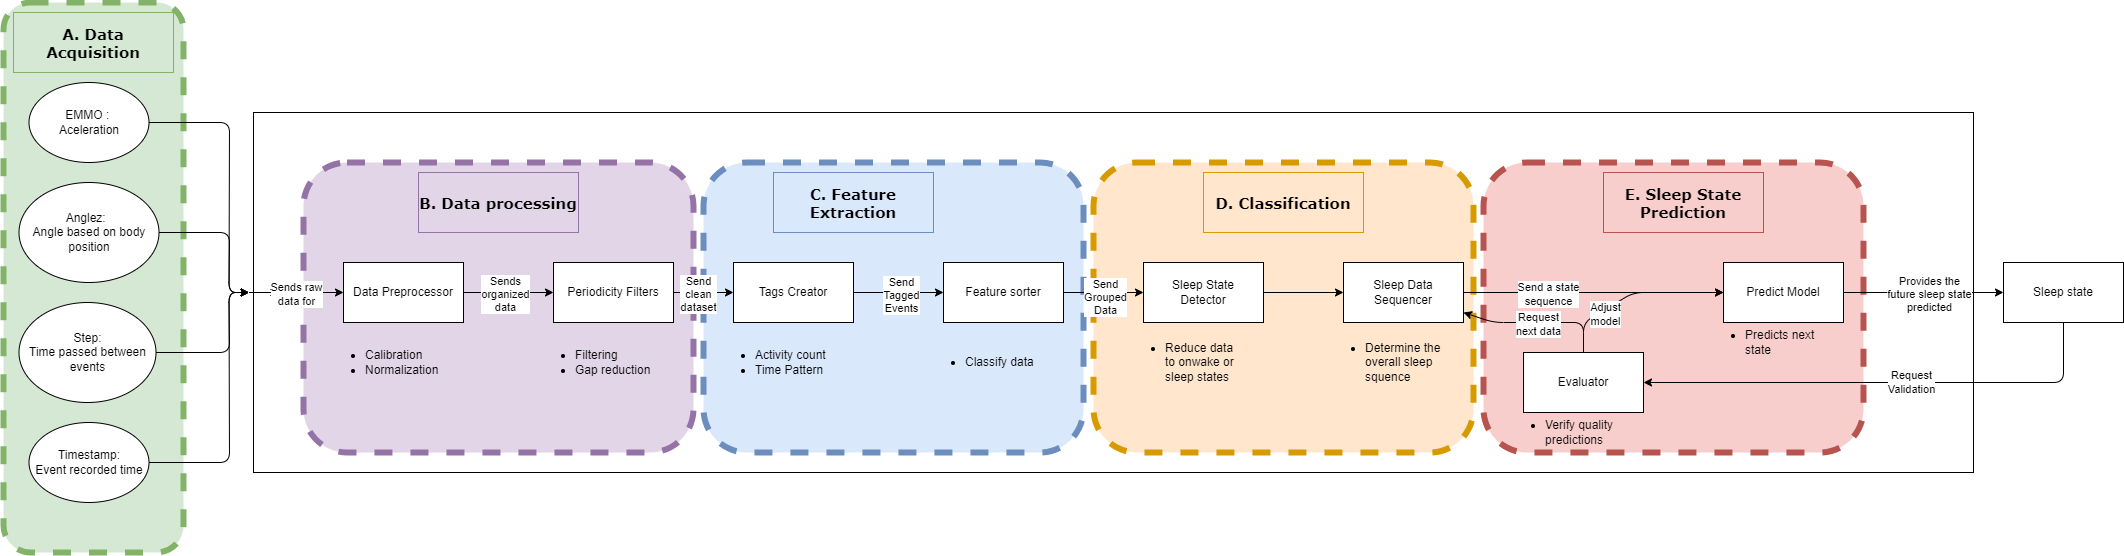
\includegraphics[width=0.85\textwidth]{system_architecture.png}
\end{center}

\vspace{0.4em}
Our solution implements a five-module pipeline: (1) Data Acquisition from wearable accelerometers, (2) Signal Processing with calibration and normalization, (3) Feature Extraction calculating activity counts, (4) Classification using traditional algorithms (Cole-Kripke, Sadeh, OPAL), and (5) LLM Enhancement via Amazon Chronos transformer. The key innovation integrates pre-trained time series foundation models to capture long-range temporal dependencies in sleep-wake cycles, providing probabilistic forecasts with uncertainty quantification.
}

% =================== SECCIÓN INFERIOR (Resultados y Conclusiones) ===================
\begin{columns}
\column{0.6}
\block{Results \& Performance Analysis}{
\begin{center}
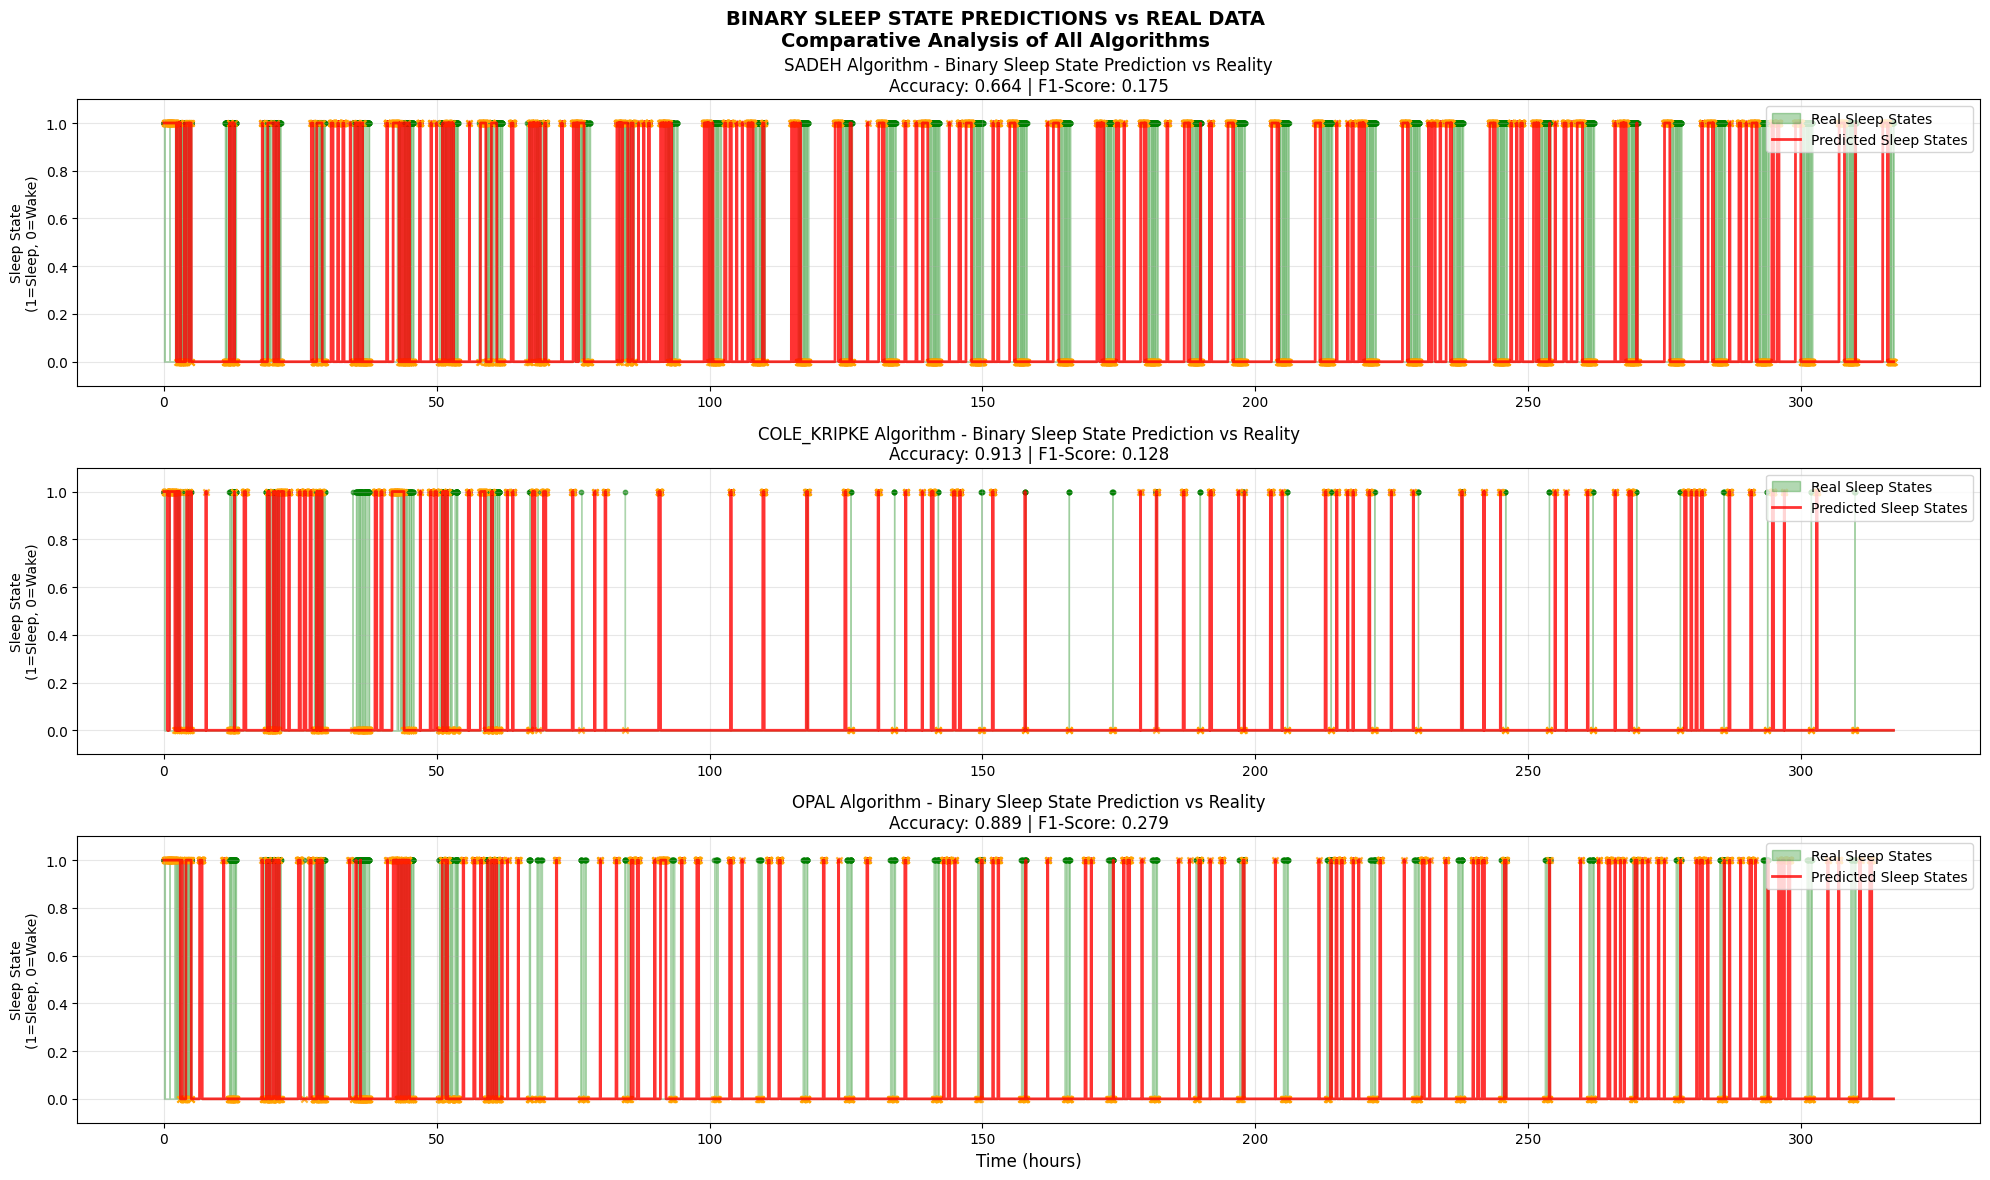
\includegraphics[width=0.55\textwidth]{llm_comparison_results.png}
\end{center}

\vspace{0.4em}
\begin{center}
\begin{tabular}{|l|c|c|c|}
\hline
\textbf{Algorithm} & \textbf{Accuracy} & \textbf{F1-Score} & \textbf{Performance} \\
\hline
Cole-Kripke + LLM & \textcolor{accent}{\textbf{91.3\%}} & 12.8\% & Best overall accuracy \\
OPAL + LLM & 88.9\% & \textcolor{accent}{\textbf{27.9\%}} & Best sleep detection \\
Sadeh + LLM & 66.4\% & 17.5\% & Enhanced fragmentation \\
\hline
\end{tabular}
\end{center}

\vspace{0.3em}
Amazon Chronos transformer demonstrated superior capability in capturing complex temporal patterns across ~300 hours of sleep data. The LLM enhancement provided probabilistic forecasts with uncertainty quantification, significantly improving prediction reliability.
}

\column{0.4}
\block{Conclusion \& Future Work}{
Our hybrid approach successfully achieved the research goal by integrating traditional actigraphy with Large Language Models for enhanced sleep state prediction. 

\vspace{0.3em}
\textbf{Key Achievements:}
\begin{itemize}
    \item Cole-Kripke + LLM: 91.3\% accuracy
    \item Real-time monitoring capabilities
    \item Uncertainty quantification
    \item Modular architecture design
\end{itemize}

\vspace{0.3em}
\textbf{Future Directions:}
\begin{itemize}
    \item Personalized algorithm calibration
    \item Wearable device integration
    \item Clinical deployment optimization
\end{itemize}
}

\block{Bibliography}{
\begin{itemize}
    \item Ansari, A.F. et al. (2024). "Chronos: Learning the Language of Time Series." Amazon Science.
    \item Cole, R.J. et al. (1992). "Automatic sleep/wake identification from wrist activity." Sleep, 15(5).
    \item Sadeh, A. et al. (1994). "Activity-based assessment of sleep-wake patterns." Sleep, 17(3).
\end{itemize}
}
\end{columns}

\end{document}